
\chapter{Introduction}
\section{Purpose}

\textbf{Data4Help} is a service whose aim is to collect eHealth data acquired from registered users and make it available for other particular users, called third parties.

\par \noindent \newline
The purpose of this document is to give an overview of Data4Help capabilities, serving as a guideline to fully understand what this system should provide to the end users. Reading this report
is essential to gather all the information needed for the software developing and testing, especially to distinguish  \textbf{what is assumed by the system} and what is \textbf{required} from it.

\par \noindent \newline
Data4Help is a system that can allow the joining of two typologies of users:
\begin{itemize}
\item Individuals that want their data to be acquired by Data4Help.
\item Third-Parties that want to access the collected data.
\end{itemize}
The system should also provide another service, built on top of Data4Help, called AutomatedSOS.
\newline
 This service monitors the health status of the subscribed user and when some parameters are below certain thresholds, sends to the customer and ambulance.
\newline
Improving users lifestyle and helping third party to analyze their health status will be the key driver of Data4Help features.
\newline
In the following chapters more details will be presented.


\section{Scope}
\subsection{Description of the given problem}
Data4Help aims to collect and gather in one place all the data related to the health condition of a registered user (steps taken daily, average heart beat, possible activities done in a day) from any device capable of collecting at least one of these kind of data.
The collected data can be accessed by third-parties in two different ways:
\begin{itemize}
\item Anonymized data: data of group of individuals, where the group can be identified by location, parameters on specific data (both on the user and the collected data). To maintain a certain level of privacy requests that select groups that count higher than 1000 individuals are allowed by the system.
\item Specific individual data: data of a specific user, this can be accessed only after the third-party sends a request to access the user data, and the user accepts it. The handling of the request for individual data is handled by the system.
\end{itemize}
The system also updates as soon as possible the third parties, when new accessible data is gathered.
To distinguish between individuals account, and third parties account at the moment of registration the user must select what kind of account it is going to create.
Third parties can also subscribe to another service, included in the application: AutomatedSOS. This service monitors the health status of an individual continuously, and, if certain parameters go below a critical threshold, the application starts automatically a rescue procedure. The rescue procedure should start in under 5 seconds from the crossing of the treshold and consists in sending an ambulance to the position of the user.
\newline
In a fragmented market like the wearables one, Data4Help focus on organizing all the data coming these devices and provide it easily while respecting user privacy.
 \newline
This is not the only purpose of Data4Help, indeed the AutomatedSOS service enable the system to have an active role in the life of its users, monitoring their health constatly and providing them emergency support.
\subsection{World and machine phenomena}
\begin{figure}[H]
\centering
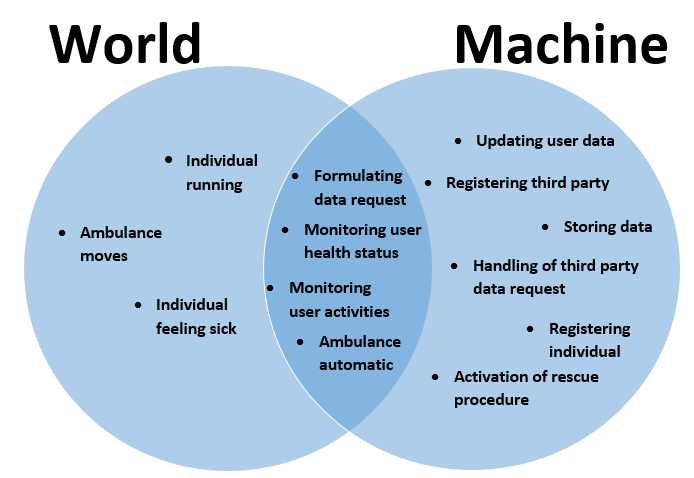
\includegraphics[scale=0.7]{resources/worldandmachine.png}
\end{figure}


\subsection{Goals}

\begin{itemize}
\item[] \goal{Individuals eHealth data is correctly gathered from their wearables.}{Data}
\item[]\goal{
Third parties can have access to accepted group data requests.
}{GroupData}
\item[]\goal{
Third parties can have access to data of specific individuals that gave permission to it.
}{SpecData}
\item[]\goal{
Third parties can receive updates whenever new data of their observed groups or individuals is gathered.
}{Notify}
\item[]\goal{
An ambulance is called whenever an individual vital parameter crosses a critical treshold.
}{Rescue}
\item[]\goal{
Users privacy is maintained.
}{Privacy}
\end{itemize}








\section{Definitions, Acronyms, Abbreviations}
\subsection{Definitions}
\begin{itemize}
\item \textbf{Rescue Procedure}: all the operations needed to save a person life. The operations include both the ones handled by computers and humans.
\item \textbf{eHealth Data}: all the data that can the related to the general health of the user, for example steps taken daily, hearth beat, blood pressure, activity level
\item \textbf{Health status}: level of health of a person, obtained analyzing various parameters like  hearthbeat rate, weight, hours of sleep.
\item \textbf{Critical Treshold}: value that, referred to an health parameter, must not be passed to guarantee user vital activities.
\end{itemize}




\subsection{Acronyms}

\begin{itemize}
\item \textbf{SSN}: Social Security Number
\item \textbf{TC}: Tax Code
\item \textbf{DBMS}: Database Management System
\item \textbf{DDoS}: Distributed Denial of Service
\item \textbf{GPS}: Global Positioning System
\end{itemize}




\section{Revision History}
\section{Reference Documents}
\section{Document Structure}